\documentclass[a4paper]{article}

\usepackage[margin=2cm]{geometry}	% For smaller margins
\usepackage[catalan]{babel} 		% Catalan language 
\usepackage{fontspec}				% utf-8 support

\usepackage{amsmath}				% Math symbols
\usepackage{float}					% Better positioning 
\usepackage[hidelinks]{hyperref}	% To hide some links
\usepackage{pgfplots}				% Useful to plot data tables
\usepackage{enumitem}				% To use resume in enumerate
\usepackage{multirow}				% Multirow
\usepackage{gensymb} 				% For the degree symbol
\usepackage{graphicx}				% To include images
\usepackage{array}					% To alter column specification

\pgfplotsset{compat=1.13}

\setlength{\parindent}{0pt}
\setlength{\parskip}{1em}

\title{
	\textsc{Laboratori de Termodinàmica} \\
	\textsc{Pràctica 4} \\
	Cicle de refrigeració per compressió de vapor amb R-134a \\
	\large
	Professor: Jose Luís \\ Grup: 11 }
\author{Jo-an Marcè Igual \and Esteve Tarragó Sanchís}
\date{13 de novembre de 2016}

\begin{document}
\maketitle

\section{Objectius}

\begin{itemize}
	\item Comprendre el funcionament d’un cicle de refrigeració.
	\item Conèixer algunes aplicacions molt usuals de cicles de refrigeració.
	\item Veure quines variables experimentals cal mesurar per tal de poder conèixer l’estat de funcionament d’un cicle frigorífic.
	\item Comprendre i utilitzar el diagrama P-h per a l’estudi del cicle
	\item Determinar la potencia tèrmica frigorífica o calorífica que proporciona el cicle i mesurar la potència elèctrica consumida necessària pel seu funcionament.
	\item Interpretar les dades que subministren els fabricants de compressors per conèixer les característiques dels cicles frigorífics.
	\item A partir de les dades experimentals es faran balanços de matèria i energia en els diferents elements de la insta\l. lació i es determinarà el coeficient de funcionament o d’eficàcia (COP) de la insta\l. lació.
\end{itemize}

\section{Presentació de resultats}

\textbf{S'ha de presentar}
\begin{enumerate}
	\item \textbf{Diagrama \emph{P-h} del cicle representat}
\end{enumerate}

\begin{figure}[H]
	\centering
	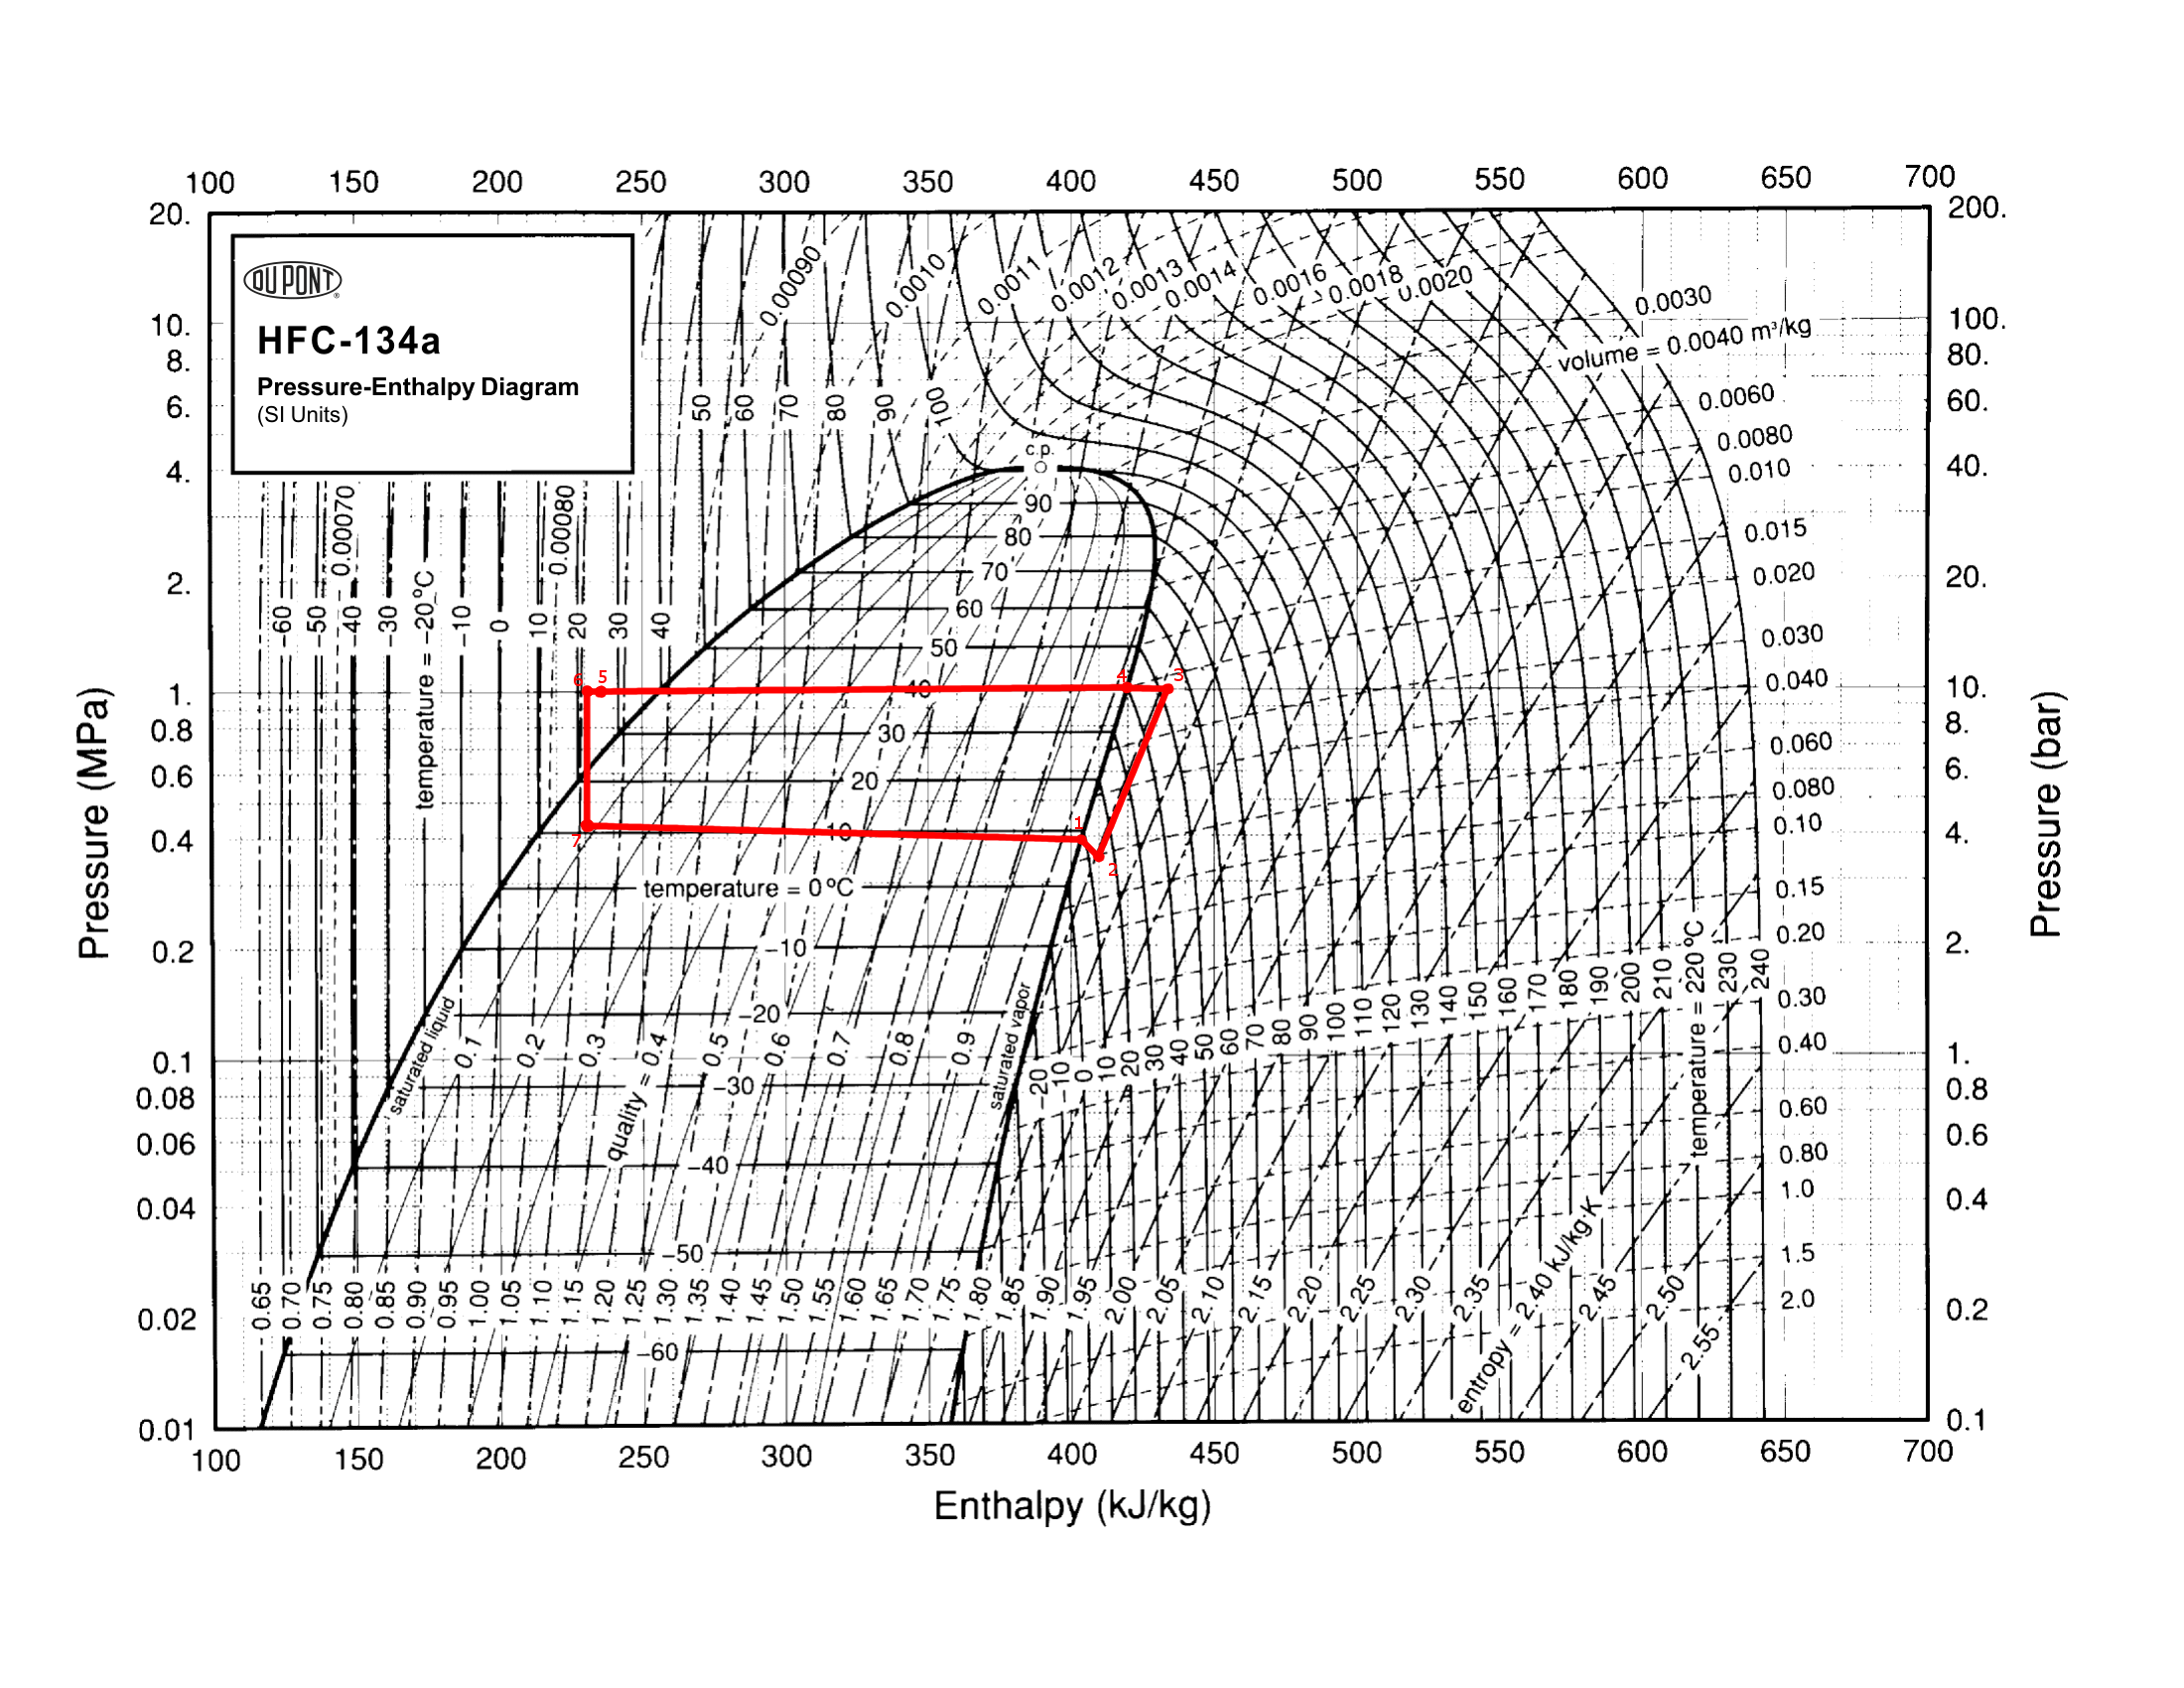
\includegraphics[width=\textwidth]{imatges/grafic-p-h.png}
\end{figure}

\begin{enumerate}[resume]
	\item \textbf{Les taules anteriorment citades en l'apartat de presa de dades amb els valors obtinguts experimentalment (que es troben també al full de resultats).}
\end{enumerate}

\begin{table}[H]
	\centering
	\begin{tabular}{l|>{\raggedleft}p{2cm}>{\raggedleft}p{1.5cm}r}
		Refrigerant & Pressió manomètrica (bar) & Pressió absoluta (bar) & Temperatura (ºC) \\
		\hline
		Sortida evaporador (1)  & 3,0 &  4,0 & Vapor Saturat \\
		Entrada compressor (2)  & 2,7 &  3,7 & 10,9 \\
		Sortida compressor (3)  & 9,0 & 10,0 & 52,7 \\
		Entrada condensador (4) & 9,0 & 10,0 & Vapor Saturat \\
		Sortida condensador (5) & 8,9 &  9,9 & 26,6 \\
		Entrada vàlvula (6)     & 8,9 &  9,9 & 24,0 \\
		Entrada evaporador (7)  & 3,1 &  4,1 & 11,5 \\
	\end{tabular}
\end{table}

\begin{table}[H]
	\centering
	\begin{tabular}{l|rr}
		Refrigerant & Pressió manomètrica (bar) & Temperatura manomètrica (ºC)\\
		\hline
		Entrada compressor & 2,7 & 6 \\
		Sortida compressor & 9,0 & 30 \\
	\end{tabular}
\end{table}

\begin{table}[H]
	\centering
	\begin{tabular}{l|rr}
		Aigua & Cabal (l/h) & Temperatura (ºC) \\
		\hline
		Entrada evaporador  & \multirow{2}{*}{110} & 23,3 \\
		Sortida evaporador  &                      & 9,0 \\
		Entrada condensador & \multirow{2}{*}{145} & 22,7 \\
		Sortida condensador &                      & 35 \\
	\end{tabular}
\end{table}

\begin{enumerate}[resume]
	\item \textbf{La taula següent a partir de les dades de l'apartat anterior, (aquesta taula es troba també en el full de resultats). Indiqueu en valor absolut el valor de les potències calorífica i frigorífica.}
\end{enumerate}

\begin{table}[H]
	\centering
	\begin{tabular}{rl|r}
		1  & Potència calorífica (costat aigua) en W     & 2070 \\
		2  & Potència frigorífica (costat aigua) en W    & 1830 \\
		3  & Diferència dels dos valors anteriors en W   &  240 \\
		4  & Potència elèctrica del vatímetre en W       &  567 \\
		5  & Temperatura condensació (del manòmetre) ºC  &   43,6 \\
		6  & Temperatura evaporació (del manòmetre) ºC   &    8 \\
		7  & Pot Frigorífica del fabricant (taules) en W & 1993,7 \\
		8  & Pot elèctrica del fabricant (taules) en W   &  579,7 \\
		9  & COP calculat com (valor 2) / (valor 4)      &    3,23 \\
		10 & COP calculat com (valor 7) / (valor 8)      &    3,44 \\
		11 & Pèrdua de calor al compressor en W          &  327,7 \\
	\end{tabular}
\end{table}

\begin{enumerate}[resume]
	\item \textbf{Un comentari o anàlisi sobre els resultats obtinguts i la coherència dels càlculs efectuats}
\end{enumerate}

Com es pot observar hi ha una diferència entre el COP del fabricant i el COP mesurat. El mesurat és relativament inferior al que hauria de ser. Aquesta diferència és proporcional a la de potència frigorífica entre el fabricant i la mesurada. Això pot ser degut pèrdues en la insta\l.lació que el fabricant no va considerar ja que depèn de cada insta\l.lació o a que el termòmetre no es troba suficientment a prop de la zona de compressió. Tot i així, el valor es troba relativament a prop del valor del fabricant com per no considerar-ho un problema. 

Cal destacar també que a la sortida del compressor la temperatura real difereix força de la temperatura manomètrica (22,7ºC). Això és degut a que el manòmetre considera només la zona de saturació però en canvi el compressor surt de la zona de saturació al incrementar la pressió, ja que altrament es podria fer malbé.





\end{document}